\documentclass[12pt]{article}
\usepackage{amsmath, amssymb}
\usepackage{graphicx}
\usepackage{booktabs}
\usepackage{geometry}
\geometry{margin=1in}
\usepackage{setspace}
\onehalfspacing

\title{Statistical Analysis of Spotify Song Valence}
\author{}
\date{}

\begin{document}

\maketitle

\section*{Introduction}

This project analyzes valence scores from a dataset of Spotify songs. Valence measures the musical positiveness conveyed by a track, ranging from 0 (most negative) to 1 (most positive). We explore the sampling distribution of valence, test hypotheses about population means, and investigate linear relationships between valence and other song features.

\section*{Part 1 — Distribution of Valence}

We examine the distribution of valence scores using three visualization methods: a histogram with density overlay, a violin plot, and a boxplot.

\begin{figure}[h!]
    \centering
    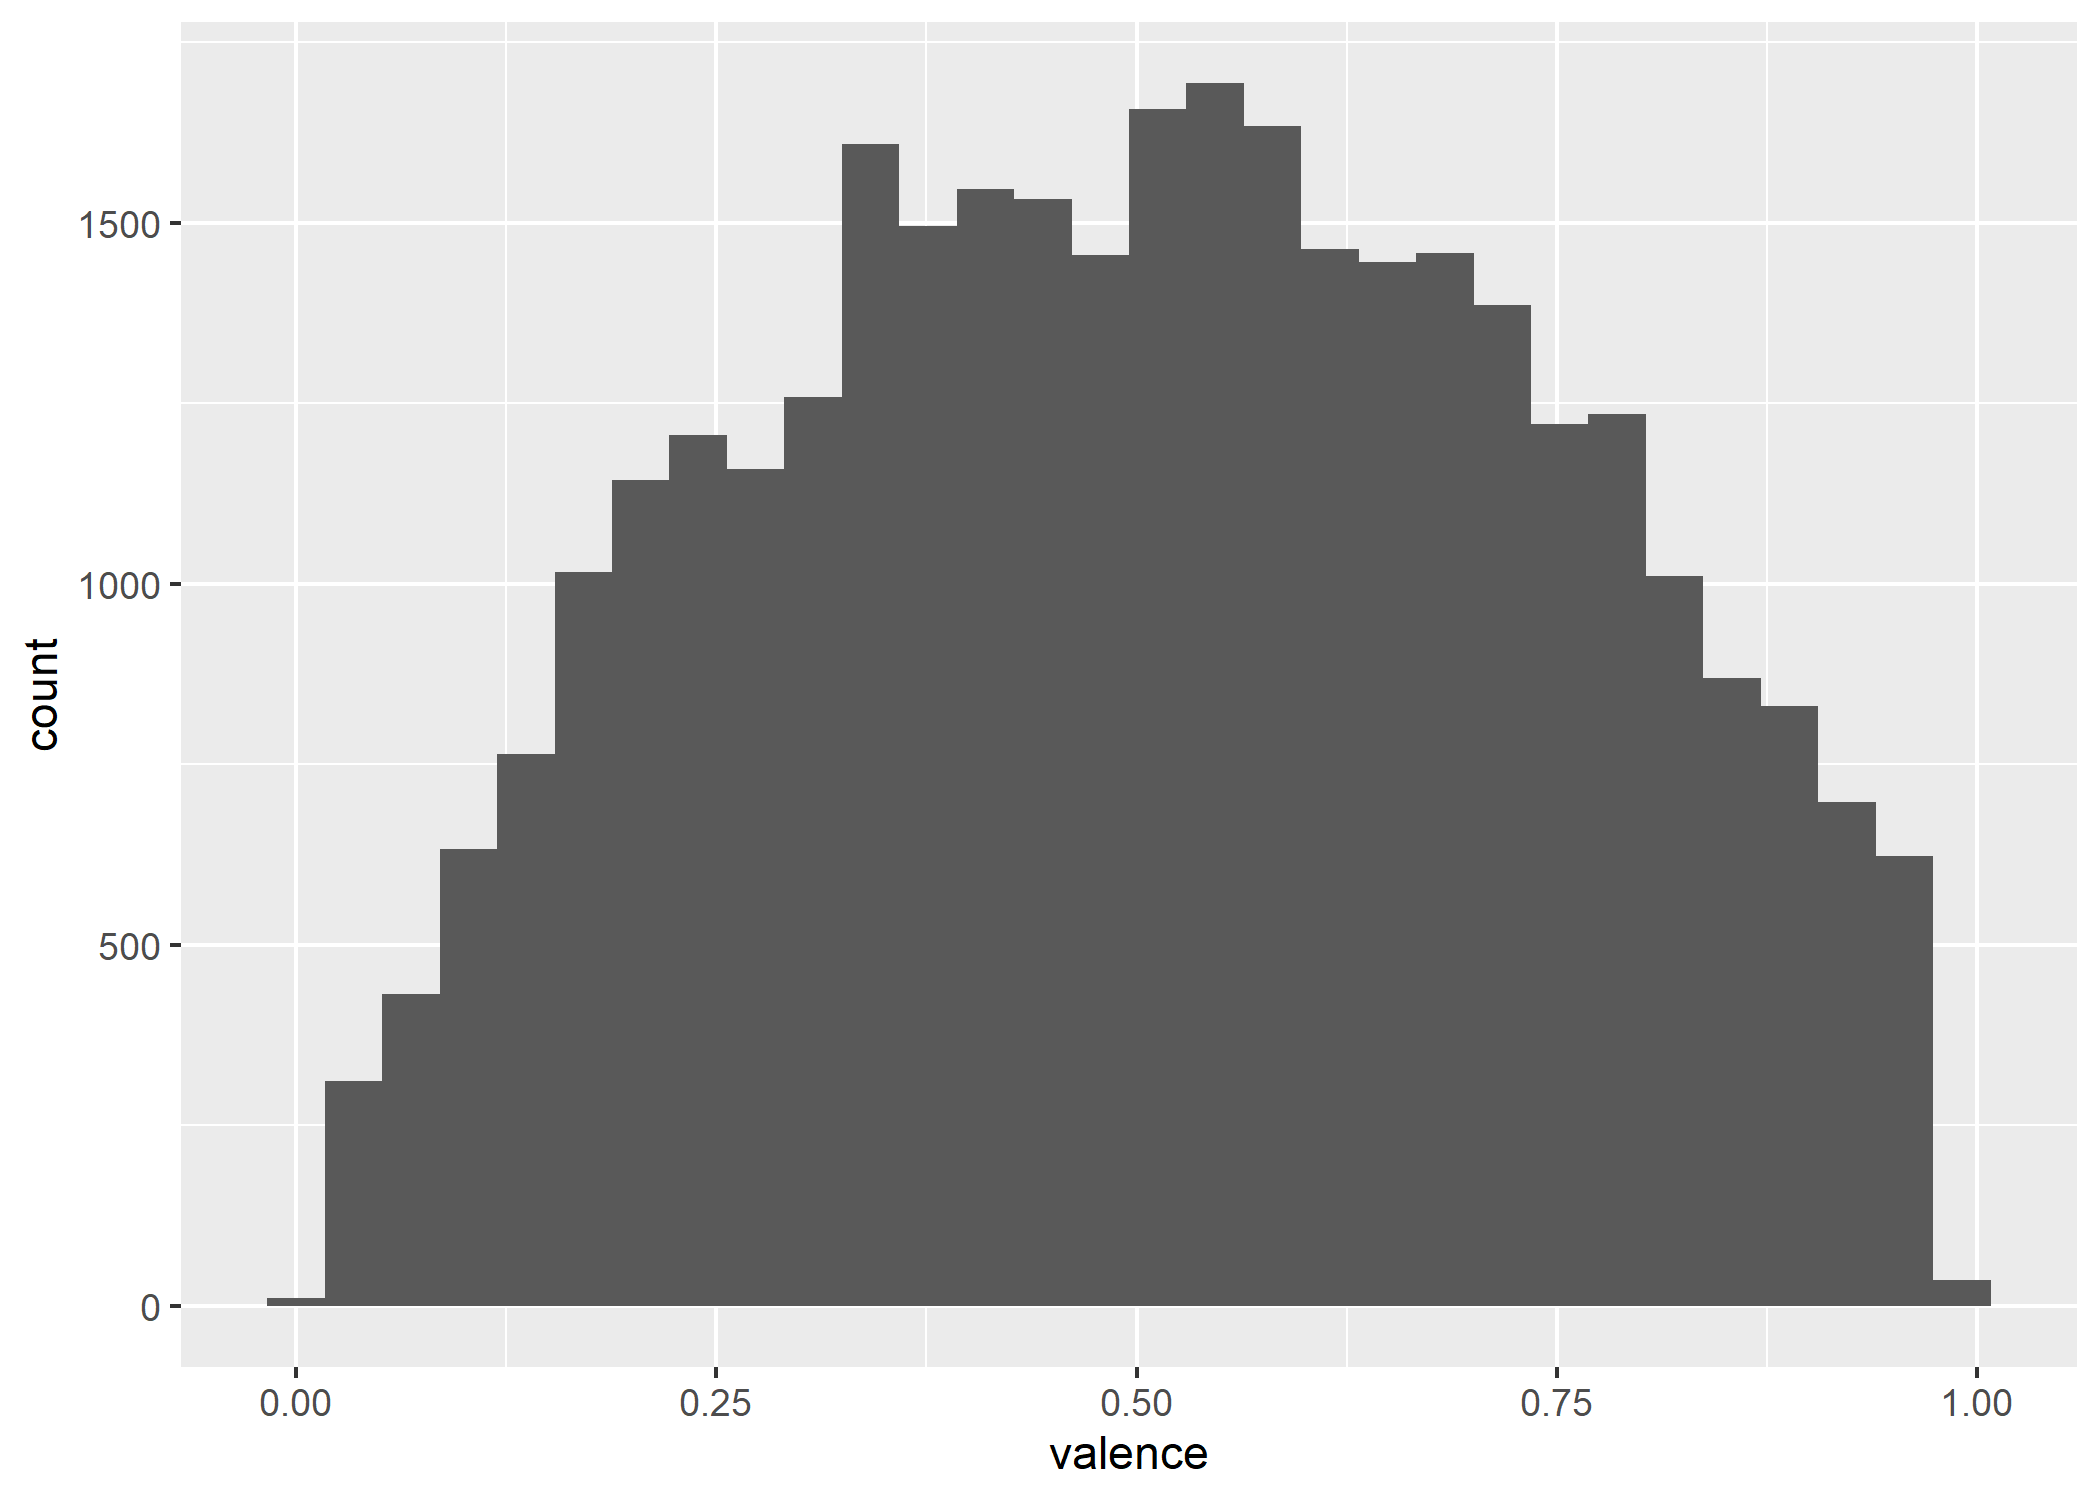
\includegraphics[width=0.8\textwidth]{histogram.png}
    \caption{Histogram of valence scores with density curve overlay.}
\end{figure}

\begin{figure}[h!]
    \centering
    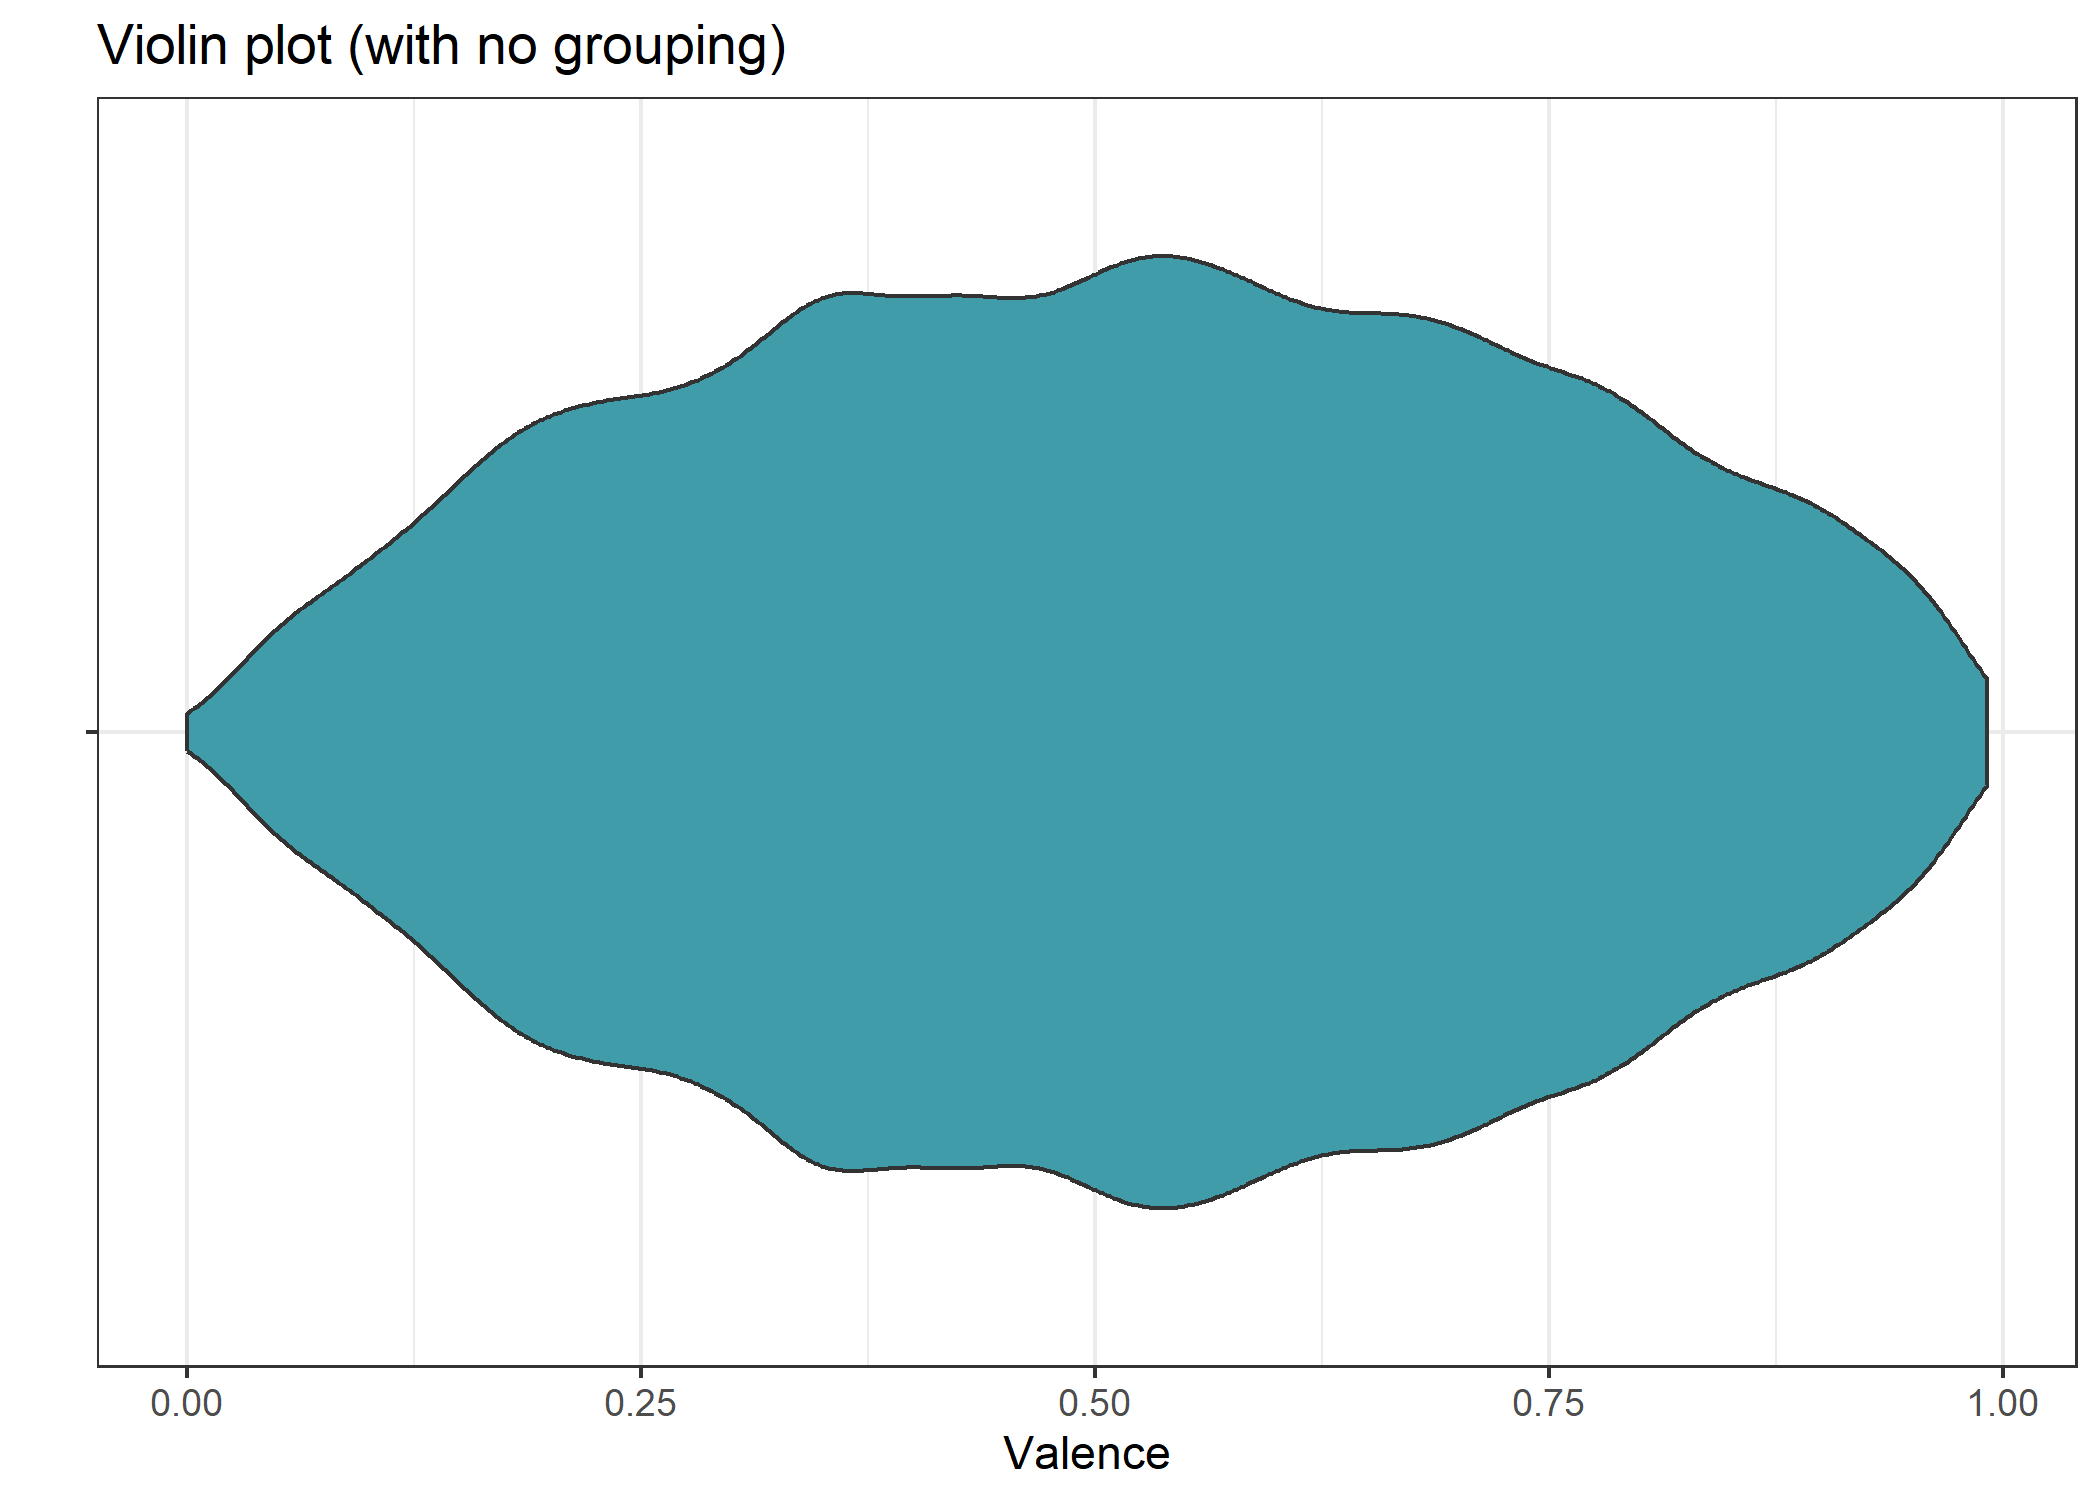
\includegraphics[width=0.8\textwidth]{violin.png}
    \caption{Violin plot of valence scores.}
\end{figure}

\begin{figure}[h!]
    \centering
    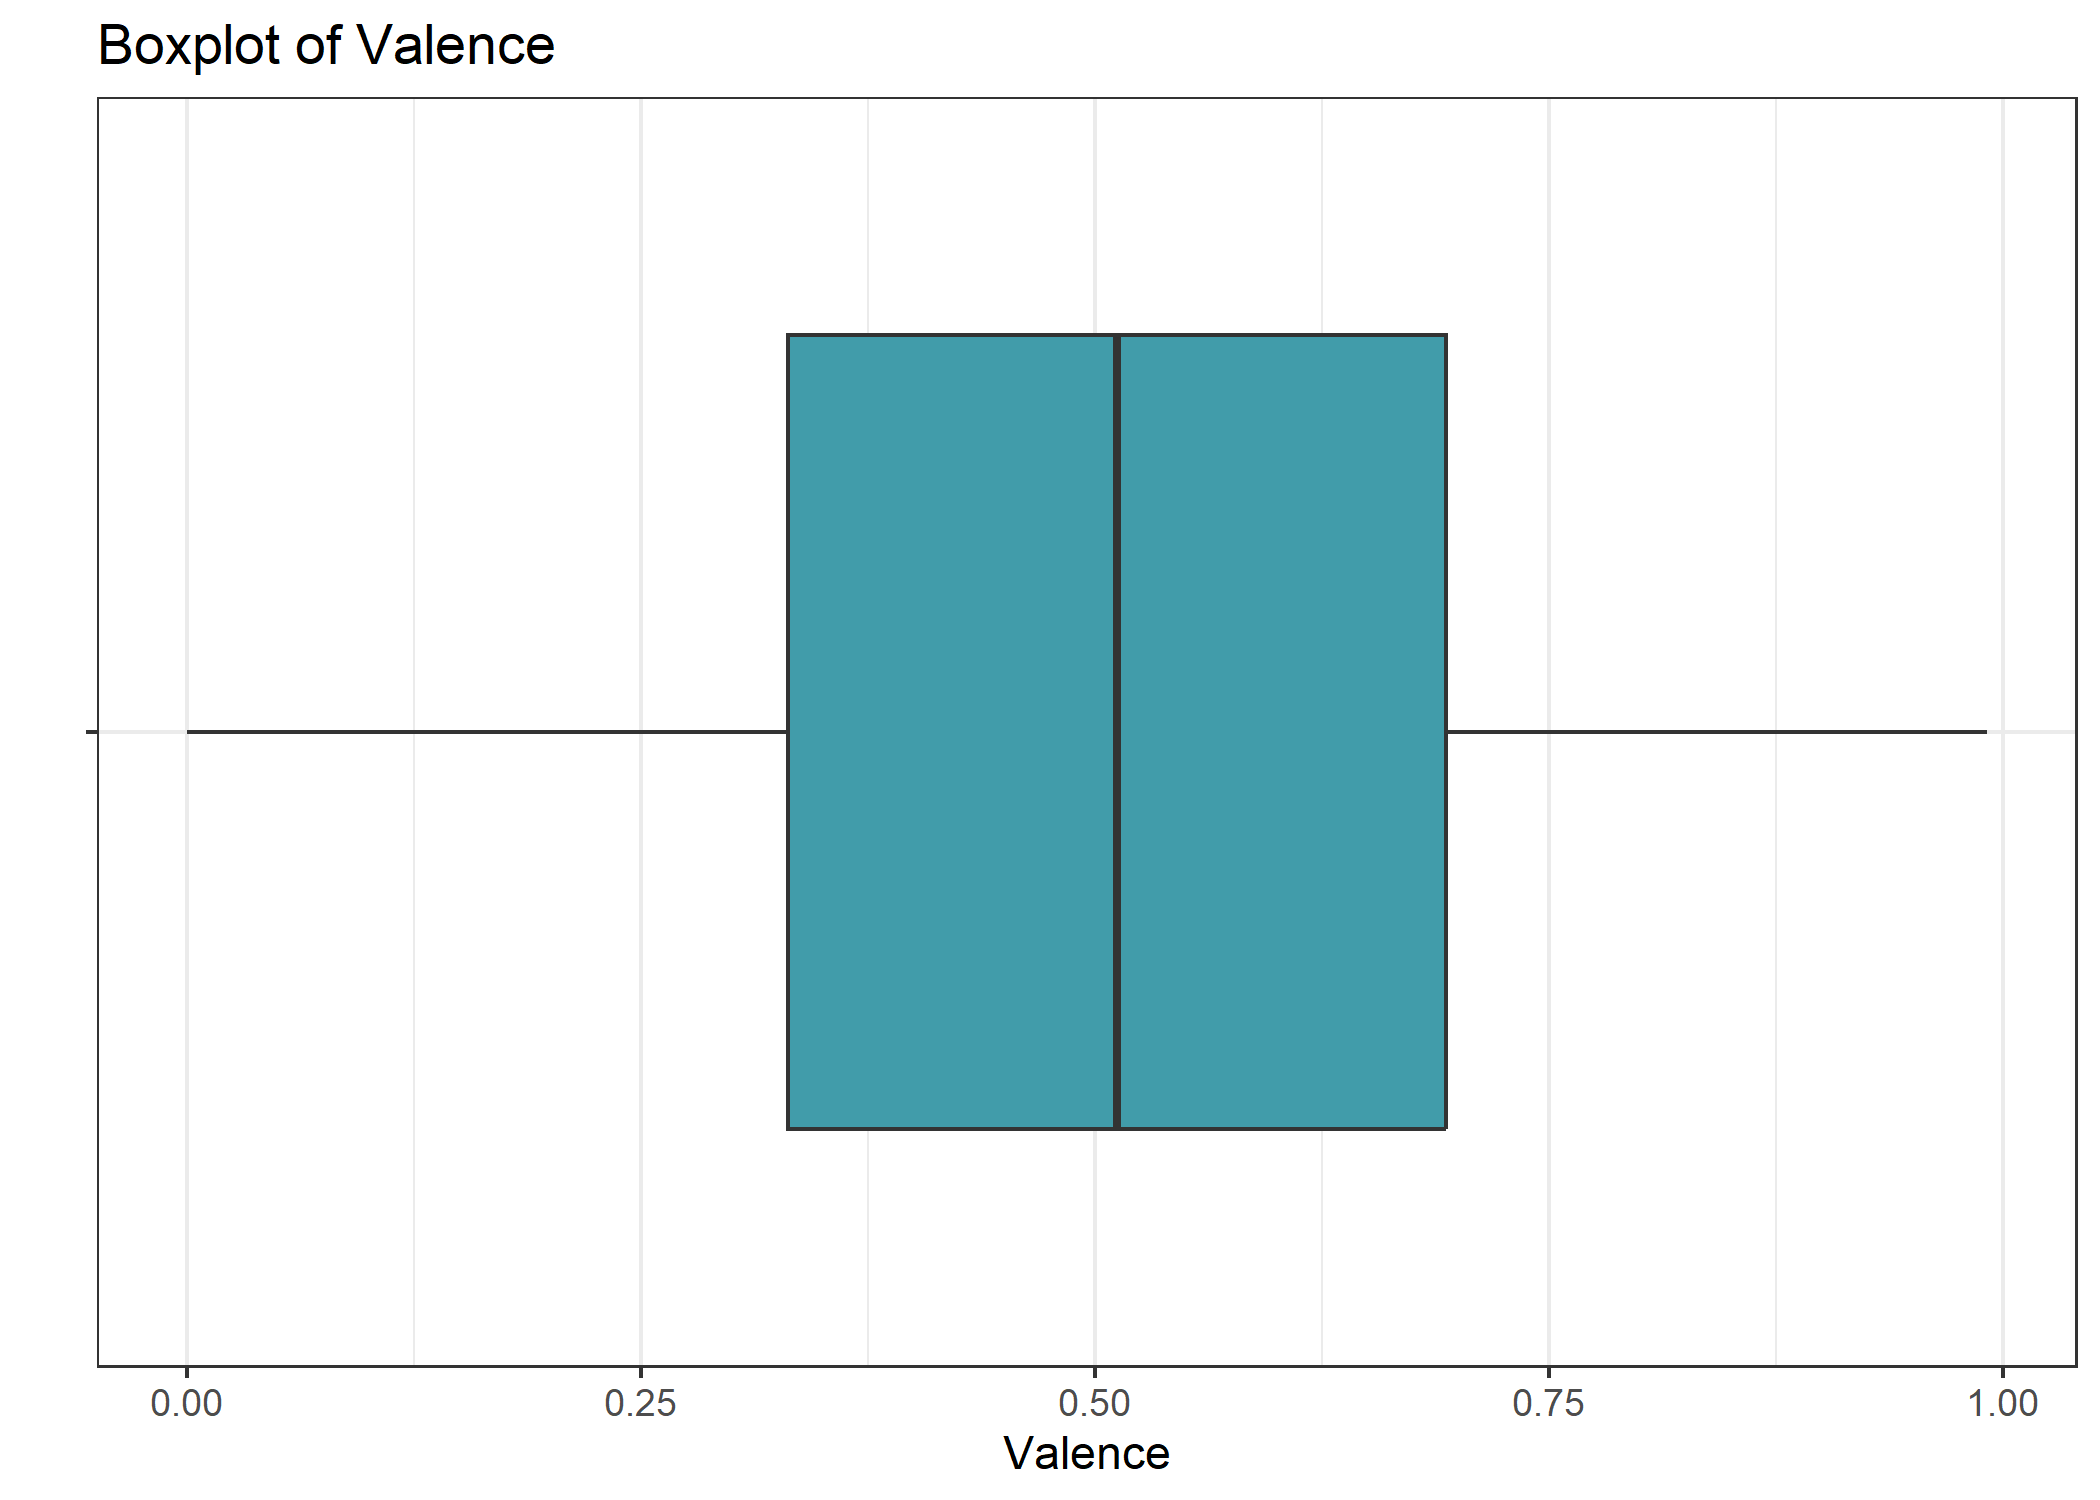
\includegraphics[width=0.6\textwidth]{boxplot.png}
    \caption{Boxplot of valence scores.}
\end{figure}

Among these three methods, the histogram with density overlay is the most informative because it shows both the frequency distribution and the shape simultaneously, while the violin plot emphasizes density at different values and the boxplot provides a compact summary but hides detail about the underlying distribution.

\subsection*{SOCS Description}

\textbf{Shape:} The distribution is nearly symmetric with a slight left skew ($-0.005$). It is unimodal and tent-shaped, flatter than a normal distribution due to the bounded range $[0, 1]$.

\textbf{Outliers:} Using the $1.5 \times \text{IQR}$ rule: $Q_1 = 0.331$, $Q_3 = 0.693$, $\text{IQR} = 0.362$. Lower fence $= Q_1 - 1.5(\text{IQR}) = -0.212$; upper fence $= Q_3 + 1.5(\text{IQR}) = 1.236$. Since all valence values fall between 0 and 1, there are no outliers.

\textbf{Center:} The mean is $\bar{x} = 0.510$ and the median is $0.512$, confirming the symmetry of the distribution. Songs have a moderate amount of musical positivity on average.

\textbf{Spread:} The standard deviation ($s = 0.2331$) and IQR ($0.362$) indicate that valence scores are fairly spread across the full $[0, 1]$ range rather than clustering tightly around the center.

\subsection*{Reflection}
The nearly uniform/tent-shaped distribution was surprising — a bell-shaped (normal) distribution was expected with most songs clustering around moderate positivity levels. Instead, valence is relatively evenly distributed across its entire range.

\section*{Part 2 — Central Limit Theorem Calculations}

The population parameters for valence are:
\[
\mu = 0.5106, \quad \sigma = 0.2331
\]

For each sample size, we draw a random sample and compute the Z-score of the sample mean (or observation):

\begin{itemize}
    \item $n = 1$: Sample value = $0.2470$, $Z = \frac{x - \mu}{\sigma} = -1.1305$
    \item $n = 10$: Sample mean = $0.4794$, $\bar{X} \sim N(\mu, \sigma/\sqrt{n})$, $Z = -0.4227$
    \item $n = 40$: Sample mean = $0.5303$, $\bar{X} \sim N(\mu, \sigma/\sqrt{n})$, $Z = 0.5348$
\end{itemize}

\section*{Part 3 — Sampling Distribution Visualization}

We simulate the sampling distribution of the sample mean by drawing 10,000 samples of size $n = 40$:

\[
\bar{X}_1, \bar{X}_2, \dots, \bar{X}_{10000}, \quad \text{where } \bar{X}_i = \frac{1}{40}\sum_{j=1}^{40} X_{ij}
\]

The observed statistics are:
\[
\begin{aligned}
    \text{Mean of sample means} &= 0.5103 \\
    \text{SD of sample means}   &= 0.0366 \\
    \text{Theoretical SE}        &= \sigma/\sqrt{n} = 0.0369
\end{aligned}
\]

\begin{figure}[h!]
    \centering
    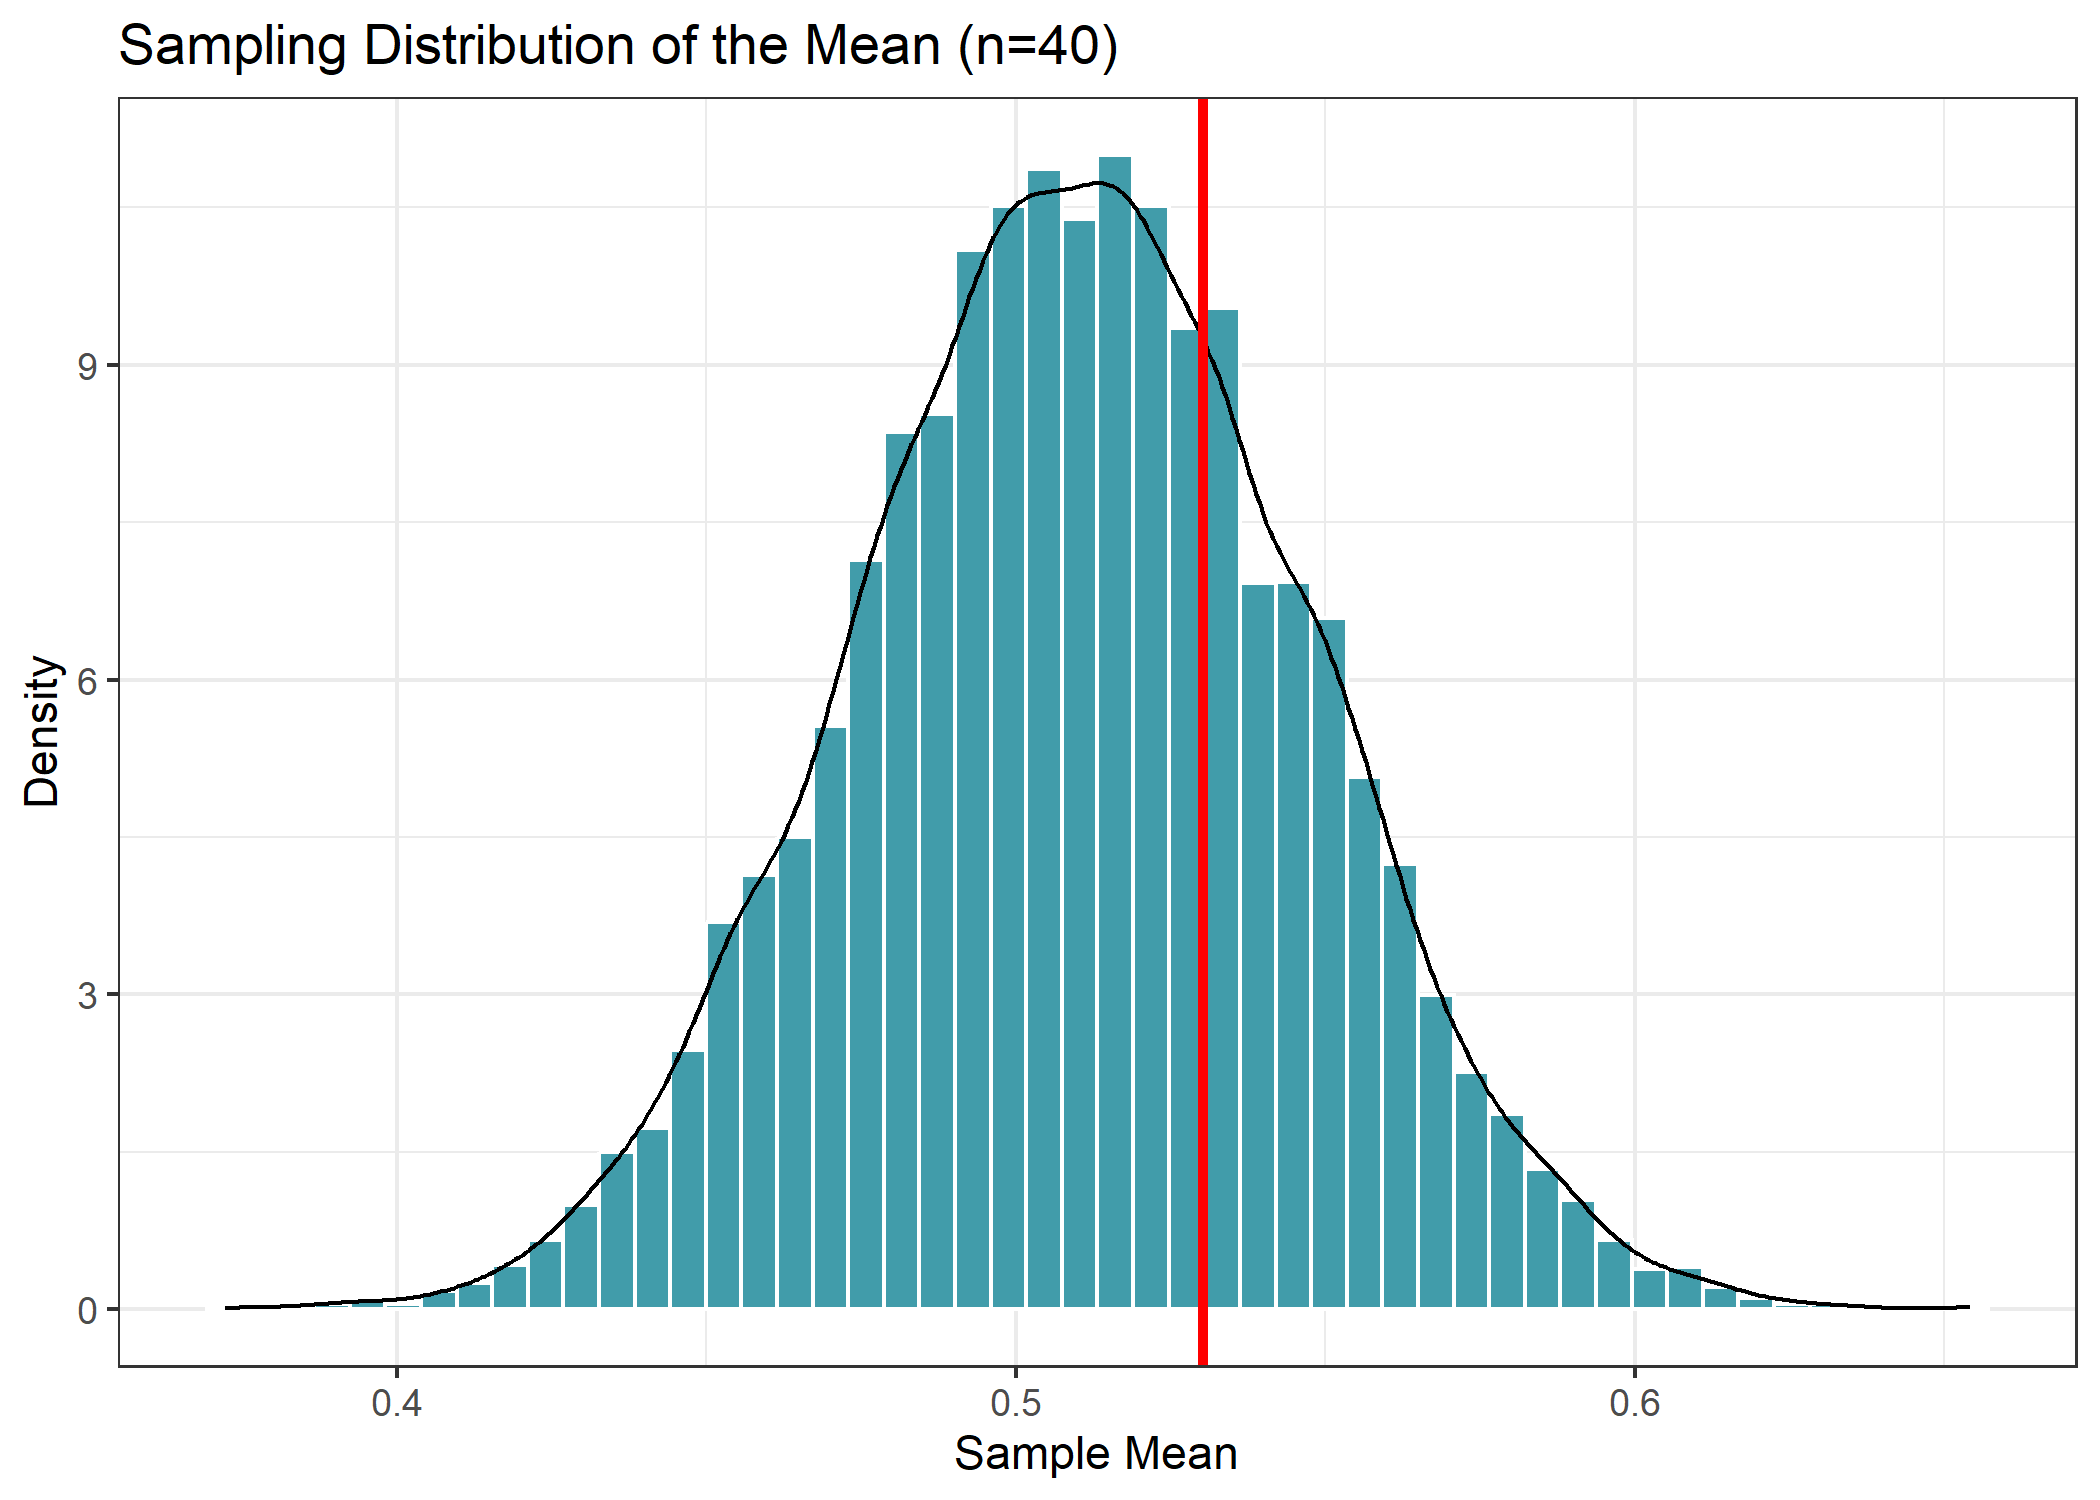
\includegraphics[width=0.8\textwidth]{samplingDist.png}
    \caption{Sampling distribution of the mean (n=40) with density overlay and red line marking the observed sample mean from Part 2.}
\end{figure}

The sampling distribution closely follows a normal curve, consistent with the Central Limit Theorem.

\section*{Part 4 — P-value and Hypothesis Testing}

We compare valence scores between two randomly selected groups to test whether their population means differ.

\subsection*{Data}
Two random samples were drawn from the population:
\[
\begin{array}{lcc}
    \toprule
    & \text{Group 1 (n=30)} & \text{Group 2 (n=35)} \\
    \midrule
    \text{Mean valence} & 0.5185 & 0.5071 \\
    \text{SD}            & 0.2299 & 0.2274 \\
    \bottomrule
\end{array}
\]

\subsection*{Hypotheses}
Let $\mu_1$ and $\mu_2$ denote the true population mean valence for Group 1 and Group 2:
\[
\begin{aligned}
    H_0 &: \mu_1 - \mu_2 = 0 \\
    H_a &: \mu_1 - \mu_2 \neq 0
\end{aligned}
\]

\subsection*{Two-Sample t-Test (Welch)}
\[
t = \frac{\bar{x}_1 - \bar{x}_2}{\sqrt{s_1^2/n_1 + s_2^2/n_2}} = 0.2015
\]
Degrees of freedom (Welch-Satterthwaite): df = $61.28$. \\
p-value: $0.841$.

\begin{itemize}
    \item At $\alpha = 0.05$, we fail to reject $H_0$ since p = $0.841 > 0.05$.
    \item The 95\% confidence interval for the difference in means is ($-0.1023$, $0.1252$), which includes zero.
\end{itemize}

\subsection*{Non-Parametric Test (Wilcoxon Rank-Sum)}
\[
W = 533.5, \quad p\text{-value} = 0.9143
\]
The conclusion is consistent with the t-test: we fail to reject $H_0$.

\subsection*{Why a t-test with n = 20 May Not Be Appropriate}
The t-test relies on the assumption that the sampling distribution of the mean is approximately normal. For small samples ($n < 30$), this approximation depends heavily on the underlying population being roughly normal. Our valence data has a tent-shaped (platykurtic) distribution, not a bell-shaped one. With only $n = 20$ per group, the Central Limit Theorem may not have taken full effect, and the t-test p-value could be unreliable. Larger samples ($n \geq 30$) provide more robustness against deviations from normality, which is why we used groups of size 30 and 35 in this analysis.

\section*{Part 5 — Linear Regression}

We investigate whether danceability is linearly related to valence using a random sample of $n = 40$ songs.

\subsection*{Data}
\[
\begin{array}{lcc}
    \toprule
    & \text{Valence (Y)} & \text{Danceability (X)} \\
    \midrule
    \text{Mean}   & 0.5303 & 0.6444 \\
    \text{SD}     & 0.2131 & 0.1415 \\
    \bottomrule
\end{array}
\]

\subsection*{Regression Model}
We fit the model: $\text{valence} = \beta_0 + \beta_1 \cdot \text{danceability} + \epsilon$

\[
\begin{array}{lcccc}
    \toprule
    \text{Coefficient} & \text{Estimate} & \text{Std.\ Error} & t\text{-value} & p \\
    \midrule
    \text{Intercept}   & 0.2696 & 0.1552     & 1.738  & 0.0904 \\
    \text{Danceability}& 0.4045 & 0.2353     & 1.719  & 0.0938 \\
    \bottomrule
\end{array}
\]

\[
R^2 = 0.0721, \quad F(1, 38) = 2.954, \quad p = 0.0938
\]

Regression equation: $\widehat{\text{valence}} = 0.2696 + 0.4045 \cdot \text{danceability}$

\subsection*{Correlation Analysis}
\[
r_{\text{sample}} = 0.2686, \quad \rho_{\text{population}} = 0.3305
\]

\subsection*{Bootstrap Confidence Interval}
Using $B = 10,000$ bootstrap replicates:
\[
90\%\text{ CI for } \rho: (0.0098, 0.4808)
\]
The true population correlation is inside the confidence interval.

\subsection*{Diagnostic Plots}
\begin{figure}[h!]
    \centering
    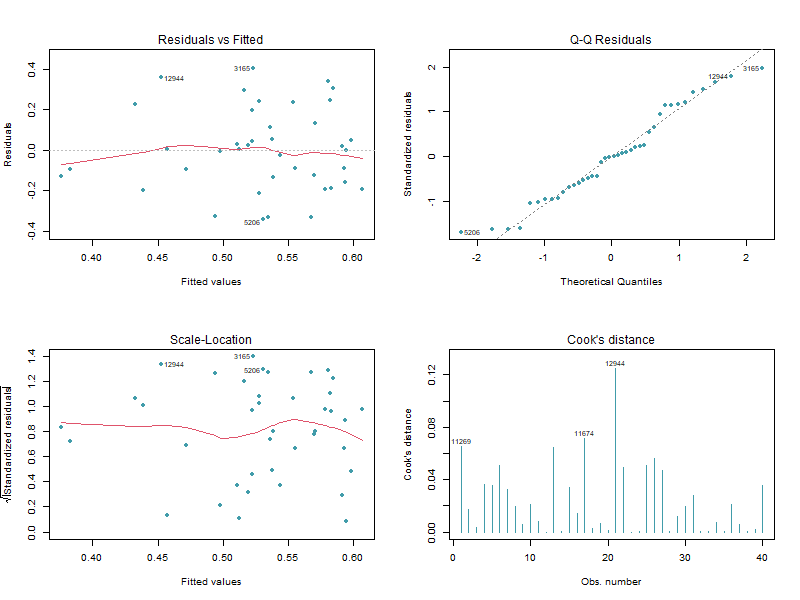
\includegraphics[width=0.8\textwidth]{diagnostics.png}
    \caption{Regression diagnostic plots: residuals vs fitted, normal Q-Q, scale-location, and residuals vs leverage.}
\end{figure}

\subsection*{Conclusion}
There is a moderate positive linear relationship between danceability and valence ($r = 0.27$, population $\rho = 0.33$). The slope approaches significance at $\alpha = 0.05$ ($p = 0.094$), and the model explains about $7\%$ of the variation in musical positivity. This suggests that songs with stronger rhythmic stability and beat consistency tend to be more musically upbeat, which aligns with the nature of dance music genres. While not statistically significant at the conventional level, this relationship is substantially stronger than any found using track popularity as a predictor.

\section*{Overall Conclusion}
The valence distribution in Spotify songs is nearly symmetric and tent-shaped rather than normal, with no outliers and moderate spread across $[0, 1]$. The Central Limit Theorem holds well for sample means at $n = 40$, producing an approximately normal sampling distribution. Comparing two random groups from the same population yielded no significant difference in mean valence ($p = 0.841$), as expected. Finally, danceability shows a moderate positive but non-significant linear relationship with valence ($R^2 = 0.07$, $p = 0.094$), suggesting that more danceable songs tend to be slightly more musically upbeat.

\end{document}
